\section{System}
\label{sec:sys}

\begin{figure}[t]
\centering
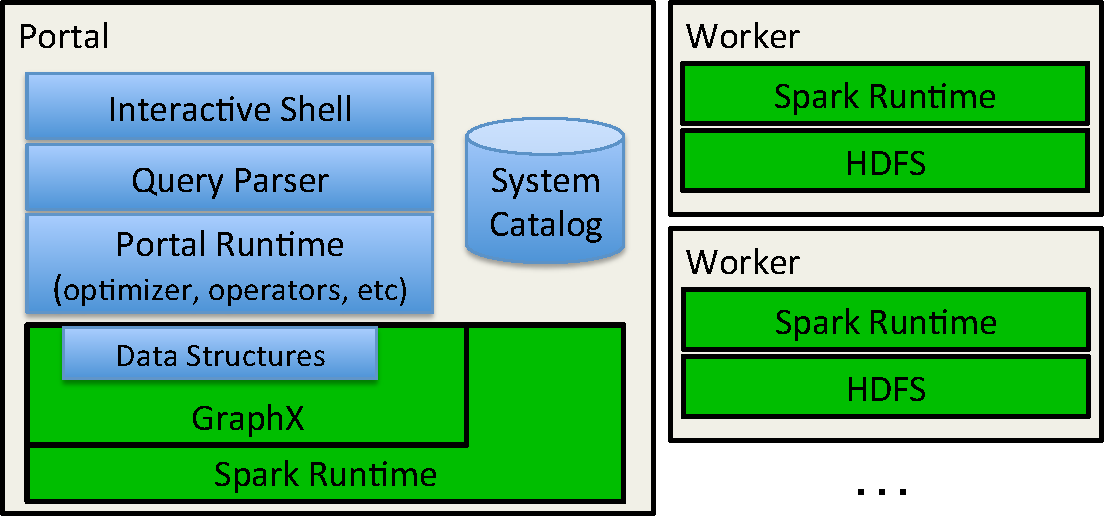
\includegraphics[width=3.4in]{figs/architecture.pdf}
\vspace{-0.4cm}
\caption{\sys system architecture.}
\vspace{-0.4cm}
\label{fig:arch}
\end{figure}

We developed a prototype system \sys which supports \tga operations on
top of Apache Spark/GraphX~\cite{DBLP:conf/osdi/GonzalezXDCFS14}, as
depicted in Figure~\ref{fig:arch}.  Green boxes indicate builtin
components, while blue are those we added for \sys.  The data is
distributed in partitions across the cluster workers, read in from
HDFS, and can be viewed both as a graph and as a pair of RDDs.  All
\tg operations are available through the public API of the \sys
library, and may be used in an Apache Spark application.

{\bf Temporal operators.}  Apache Spark is not a temporal DBMS but
rather an open-source in-memory distributed framework that combines
graph parallel and data parallel abstractions.  We reduce our temporal
operators into a sequence of nontemporal relational operators or their
equivalents for Spark RDDs, maintaining point semantics.  In some
cases, such as temporal window node creation, access methods based on
GraphX graphs provide significantly more efficient performance.  For
analytics, we use the GraphX Pregel library, but add a batching method
to compute overall time instances together
(see~\cite{MoffittTempWeb16} for a detailed discussion).  \sys
supports PageRank, connected components, and shortest paths analytics
out of the box and provides an API for adding others.  We are in the
process of adding the clustering coefficient analytic.

{\bf Query evaluation.}  \sys query execution follows the traditional
query processing steps: parsing, logical plan generation and
verification, and physical plan generation. \sys re-uses and extends
SparkSQL abstractions for these steps.  A \ql query is rewritten into
a sequence of operators, and some operators are reordered to improve
performance.  For example, pushing slice generally improves
performance similar to pushing selection in SQL.

\eat{For example, pushing temporal aggregation
  before temporal join can sometimes lead to better performance. A
  temporal join query may be rewritten to include additional temporal
  selection conditions, based on information about the temporal schema
  of the TGraphs being joined, which in turn significantly reduces
  data load time.}

We developed several different physical representations and
partitioning strategies that are selected at the physical plan
generation stage. The TGraphs are read from the distributed file
system HDFS and processed by Spark Workers, with the tasks assigned
and managed by the runtime.

\begin{figure}[t]
\centering
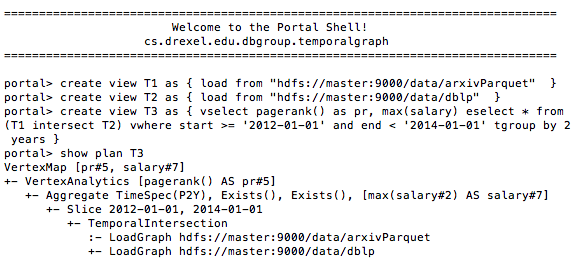
\includegraphics[width=3.4in]{figs/shell.png}
\caption{\sys interactive shell.}
\label{fig:shell}
\end{figure}

{\bf Interactive shell. Integration with SQL.}  The \sys system
includes an interactive shell for exploratory data analysis
(Figure~\ref{fig:shell}). Shell users can define (materialized) views,
inspect query execution plans and execute SQL queries with an embedded
\sys view. Consider the following SQL query that returns \insql{vid}
and \insql{tr} values of 20 vertices with the most significantly
increasing pagerank trend.

\begin{small}
\begin{verbatim}
Select VF.vid, VF.tr
From T5.vertices() as VF
Order by tr
Limit 20
\end{verbatim}
\end{small}

An important part of the query is the use of \insql{T5.vertices()} in
the From clause. This is an operation provided by the \sys
framework, which takes all the vertices of T5 and their attributes in
a single nested relation VF with schema \insql{(vid:long, start:date,
  end:date, tr:float)}. VF can be used in SQL queries. \sys also
provides an operation \insql{edges()} that returns the edges of the
graph.



